% The probabilistic lower bound for M_k (generated by a script).
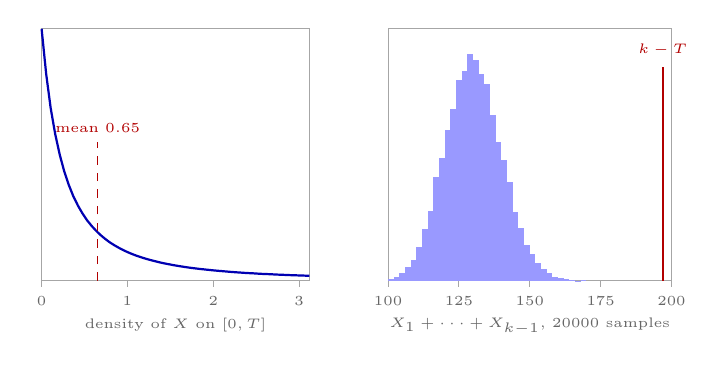
\begin{tikzpicture}[x=1cm,y=1cm]
\draw[black!35] (0,0) rectangle (3.40,3.20);
\draw[blue!70!black,thick] (0.000,3.200) -- (0.058,2.626) -- (0.115,2.194) -- (0.173,1.861) -- (0.231,1.598) -- (0.288,1.387) -- (0.346,1.215) -- (0.403,1.073) -- (0.461,0.955) -- (0.519,0.855) -- (0.576,0.770) -- (0.634,0.698) -- (0.692,0.635) -- (0.749,0.580) -- (0.807,0.532) -- (0.864,0.489) -- (0.922,0.452) -- (0.980,0.419) -- (1.037,0.389) -- (1.095,0.362) -- (1.153,0.338) -- (1.210,0.316) -- (1.268,0.297) -- (1.325,0.279) -- (1.383,0.263) -- (1.441,0.248) -- (1.498,0.234) -- (1.556,0.221) -- (1.614,0.210) -- (1.671,0.199) -- (1.729,0.189) -- (1.786,0.180) -- (1.844,0.171) -- (1.902,0.163) -- (1.959,0.156) -- (2.017,0.149) -- (2.075,0.143) -- (2.132,0.137) -- (2.190,0.131) -- (2.247,0.126) -- (2.305,0.121) -- (2.363,0.116) -- (2.420,0.111) -- (2.478,0.107) -- (2.536,0.103) -- (2.593,0.099) -- (2.651,0.096) -- (2.708,0.093) -- (2.766,0.089) -- (2.824,0.086) -- (2.881,0.084) -- (2.939,0.081) -- (2.997,0.078) -- (3.054,0.076) -- (3.112,0.073) -- (3.169,0.071) -- (3.227,0.069) -- (3.285,0.067) -- (3.342,0.065) -- (3.400,0.063);
\draw[red!70!black,dashed] (0.713,0)--(0.713,1.76) node[above,font=\tiny]{mean $0.65$};
\draw[black!35] (0.00,0)--(0.00,-0.08) node[below,font=\tiny,black!60]{$0$};
\draw[black!35] (1.09,0)--(1.09,-0.08) node[below,font=\tiny,black!60]{$1$};
\draw[black!35] (2.18,0)--(2.18,-0.08) node[below,font=\tiny,black!60]{$2$};
\draw[black!35] (3.27,0)--(3.27,-0.08) node[below,font=\tiny,black!60]{$3$};
\node[below,font=\tiny,black!60] at (1.70,-0.35) {density of $X$ on $[0,T]$};
\draw[black!35] (4.40,0) rectangle (8.00,3.20);
\fill[blue!40] (4.400,0) rectangle (4.472,0.023);
\fill[blue!40] (4.472,0) rectangle (4.544,0.042);
\fill[blue!40] (4.544,0) rectangle (4.616,0.100);
\fill[blue!40] (4.616,0) rectangle (4.688,0.176);
\fill[blue!40] (4.688,0) rectangle (4.760,0.264);
\fill[blue!40] (4.760,0) rectangle (4.832,0.424);
\fill[blue!40] (4.832,0) rectangle (4.904,0.658);
\fill[blue!40] (4.904,0) rectangle (4.976,0.890);
\fill[blue!40] (4.976,0) rectangle (5.048,1.312);
\fill[blue!40] (5.048,0) rectangle (5.120,1.554);
\fill[blue!40] (5.120,0) rectangle (5.192,1.915);
\fill[blue!40] (5.192,0) rectangle (5.264,2.178);
\fill[blue!40] (5.264,0) rectangle (5.336,2.553);
\fill[blue!40] (5.336,0) rectangle (5.408,2.662);
\fill[blue!40] (5.408,0) rectangle (5.480,2.880);
\fill[blue!40] (5.480,0) rectangle (5.552,2.804);
\fill[blue!40] (5.552,0) rectangle (5.624,2.630);
\fill[blue!40] (5.624,0) rectangle (5.696,2.495);
\fill[blue!40] (5.696,0) rectangle (5.768,2.110);
\fill[blue!40] (5.768,0) rectangle (5.840,1.762);
\fill[blue!40] (5.840,0) rectangle (5.912,1.533);
\fill[blue!40] (5.912,0) rectangle (5.984,1.248);
\fill[blue!40] (5.984,0) rectangle (6.056,0.879);
\fill[blue!40] (6.056,0) rectangle (6.128,0.673);
\fill[blue!40] (6.128,0) rectangle (6.200,0.448);
\fill[blue!40] (6.200,0) rectangle (6.272,0.341);
\fill[blue!40] (6.272,0) rectangle (6.344,0.223);
\fill[blue!40] (6.344,0) rectangle (6.416,0.149);
\fill[blue!40] (6.416,0) rectangle (6.488,0.093);
\fill[blue!40] (6.488,0) rectangle (6.560,0.053);
\fill[blue!40] (6.560,0) rectangle (6.632,0.037);
\fill[blue!40] (6.632,0) rectangle (6.704,0.016);
\fill[blue!40] (6.704,0) rectangle (6.776,0.012);
\fill[blue!40] (6.776,0) rectangle (6.848,0.002);
\fill[blue!40] (6.848,0) rectangle (6.920,0.004);
\draw[red!70!black,thick] (7.888,0)--(7.888,2.72) node[above,font=\tiny]{$k-T$};
\draw[black!35] (4.40,0)--(4.40,-0.08) node[below,font=\tiny,black!60]{$100$};
\draw[black!35] (5.30,0)--(5.30,-0.08) node[below,font=\tiny,black!60]{$125$};
\draw[black!35] (6.20,0)--(6.20,-0.08) node[below,font=\tiny,black!60]{$150$};
\draw[black!35] (7.10,0)--(7.10,-0.08) node[below,font=\tiny,black!60]{$175$};
\draw[black!35] (8.00,0)--(8.00,-0.08) node[below,font=\tiny,black!60]{$200$};
\node[below,font=\tiny,black!60] at (6.20,-0.35) {$X_1+\cdots+X_{k-1}$, $20000$ samples};
\end{tikzpicture}
